% @Author: AnthonyKenny98
% @Date:   2020-04-08 10:33:04
% @Last Modified by:   AnthonyKenny98
% @Last Modified time: 2020-04-08 11:30:28
\begin{figure}[H]
\begin{centering}
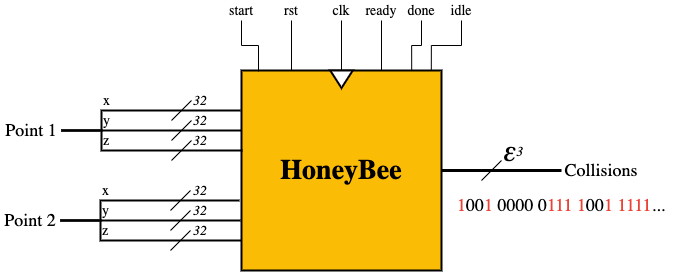
\includegraphics[width=0.8\linewidth]{chapters/chapter3/img/honeybee_interface_detail.png}
\mycaption{Port Diagram of HoneyBee Interface}{. The edge input is represented by 6 32-bit floats, following the IEEE 754 Single Precision 32-bit protocol, each float representing one of its coordinate points. The output sequence of collisions is a $e^3$-bit sequence, with each bit in the sequence representing one of the grids that was checked for intersections. It has input control signals for start and reset, and output control signals for done, idle, and ready. These control signals make up the necessary signals for a handshake protocol between HoneyBee and a processor's main controller.}
\label{fig:honeybee_interface_detail}
\end{centering}
\end{figure}